\documentclass[11pt,a4paper]{scrartcl}
\usepackage[english]{babel}
\usepackage[utf8]{inputenc}
\usepackage[T1]{fontenc}
\usepackage{lmodern}
\usepackage{amsmath}
\usepackage{amsthm}
\usepackage{amssymb}
\usepackage{enumitem}
\usepackage[hidelinks]{hyperref}
\usepackage{graphicx}
\usepackage{listings}
\usepackage{placeins}

\graphicspath{{./Figures/}}

\newtheorem*{theorem}{Theorem}
\theoremstyle{definition}
\newtheorem*{definition}{Definition}

\setlength{\parindent}{0cm}
\title{Machine Learning Final Project}
\subtitle{Seq2seq Model}
\author{Siyang Sun, Kevin Xie}
\date{\today}

\begin{document}
\begin{titlepage}
	\centering
	{\Huge\bfseries Insights into Seq2seq Models for Text Correction\par}
	\vspace{7cm}
	{\LARGE\itshape Kevin Xie (UID: 304402775)\par}
	\vspace{.9em}
	{\LARGE\itshape Siyang Sun (UID: 504400191)\par}
	\vspace{.9em}


	\vfill

\end{titlepage}
\tableofcontents

\section{Introduction}

Spellcheckers have been around since the dawn of the Information Age. This idea of an automated process to correct human spelling errors came naturally with the budding use of computers. The original spellcheckers simply accessed a list of accepted words, and checked if each word in the checked passage was a member of that list. The famous Microsoft Word spellchecker still used a predetermined dictionary, but allowed users to add their own custom words. However, as typing on computers, mobile phones, and other electronic devices became more ubiquitous, spellcheckers had to get smarter. They needed to keep up with each user’s individual typing habits and frequency of word use, and take into account the layout of the keyboard. From here, we have autocorrection software. These require machine learning and a much smarter algorithm than simply checking a static list of allowed words. In this paper, we will be building our own spellchecker using recurrent neural networks and natural language processing. We decided to create a smarter traditional spellchecker to correct errors rather than an autocorrection software that can figure out what we meant to text to our friends. This means we will train our model with correctly spelled words and correctly arranged sentences, in order to check for proper English.\newline

In this paper, we will first discuss our model and methods, and tackle the mathematics behind recurrent neural networks in the sequence-to-sequence model. Then, we will dive deeper into the algorithm we used to generate the model and build the spellchecker. After going over the results, we will discuss difficulties, improvements, and further investigation.

\section{Seq2seq Model}

To obtain our model, we used a grid search to find the optimal hyperparameters and overall architecture. Hyperparameters can include constraints, weights, or training rates. This entails an exhaustive search of a predetermined subset in the hyperparameter space to find the “best” set of hyperparameters.\newline

We will be using recurrent neural networks for our spellchecker. Specifically, we will be using a sequence-to-sequence model to do this. A sequence-to-sequence model’s two bidirectional RNNs consists of an encoder and a decoder, often used for translating between two languages. 
In this model, the encoder reads a sentence and converts it into a vector. The decoder then defines a probability of the translation based on that vector. It accomplishes this by expressing the joint probability as a product of conditional probabilities. The encoder and decoder are trained together in order to maximize the probability of an accurate translation, or in this case, spelling correction.\newline

In detail, the encoder generates a high-dimensional feature vector $c$ from the sequence of input vectors. Let $h_t$ be a hidden state at time $t$ which depends on $x_t$ and the previous state, $h_{t-1}$. $f$ is some nonlinear function such that $h_t = f(x_t, h_{t-1})$. Then $c$ is generated by some nonlinear function$q$ of all the $h_t$s. \newline

The decoder predicts the next word $y_t$ based on the words leading up to it and the context vector $c$. The joint probability of the entire segment of words $y$ is determined by the product of the conditional probabilities. \newline

The conditional probabilities are also mapped by some nonlinear function $g$. With $s_t$ as a hidden state for the decoder at time $t$, we can rewrite each conditional probability as

\[p(y_i | y_1,\dots,y_{i-1}, \textbf{x}) = g(y_{i-1},s_i,c_i).\]

We will then use these \textit{s} and the previously calculated \textit{h} to get our context vector. The nonlinear function we will use is a weighted sum, where the weights are similar to a softmax function. \newline

\section{Algorithm}
Our algorithm to solve the seq2seq model is based Tensorflow for two functions: build\_model() and train\_model(). Before we interact with these functions we must first cultivate our data. We found 22 books in ASCII and cleaned them of any open source terms of use paragraphs which usually precede the actual book. Then we went line by line and removed any occurrence of “\textasciitilde<>\{\}[]*” which are garbage values and should not be in the book. We also forced two or more spaces to one as this sometimes occurs during book scanning. Finally we separately the books into sentences.\newline

\FloatBarrier
\begin{table}
\begin{center}
\begin{tabular}{ |c|c|} 
\hline
\textbf{mean} & 149.449326 \\
\hline
\textbf{std} & 158.554753 \\
\hline
\textbf{min} & 1.000000 \\
\hline
\textbf{25\%} & 59.000000 \\
\hline
\textbf{50\%} & 111.000000 \\
\hline
\textbf{75\%} & 190.000000 \\
\hline
\textbf{max} & 8987.000000 \\
\hline
\end{tabular}
\caption{Data set statistics} 
\label{datastats}
\end{center}
\end{table}

Before we fed these cleaned sentences into our model we made sure to remove lengths that were too long as this would make our training time increase severely. Looking at Table \ref{datastats}, we see that a majority of sentences fall below 111 characters long. We set this as our max length. For the min length we set it as 9 because most simple sentences seemed to hit at least that threshold. One could set the min length anywhere between 8-15 and achieve similar results. We then simulated errors in these sentences using a function called error\_producer() at a 12\% rate by iterating through each letter in the sentence and assigning a 3\% chance that the letter will be swapped with it’s neighbor, 3\% chance the letter will be replaced by another letter, 3\% a letter will be added between the letter and its neighbor, and a 3\% chance the letter will be deleted.

\subsection{build\_model.py}
Now we can build our model. One important thing to note, the seq2seqmodel() function has the encoding and decoding RNN hidden inside its implementation. The implementation itself is boilerplate and can be found in many variations of the same template online.
\lstinputlisting[language=Python]{buildmodel.py}
\vspace{1em}
\subsection{train\_model.py}
To train our model we must feed it in batches. This is why we originally set our sentence length between 11 and 111 characters long. Seq2seq models are most efficient when they have a set length for text translation i.e. the batch size. The batch size for our final test run was 120 characters. Training a model is done in epochs which is an iteration through the entire data set. We set our max\_epoch constant to 10 but it never reached past 3.\newline

\lstinputlisting[language=Python]{trainmodel.py}
\vspace{1em}
In summary, the algorithm works to minimize an error function, in this case the cross-entropy error function, by recurrently iterating through the batches and recalculating the weight vectors until they are optimized for the data set. The min is not guaranteed to be a global min since we stop after 3 iterations through the batches.

\section{Results}
We fed the model 22 books five times for a total of 110 books. Duplicating the data was not an issue as error\_producer() is entirely random. We ran the setup on a Tesla K80 GPU with 4992 NVIDIA CUDA cores. The algorithm ran for about 80 minutes. To establish a passing grade for our model, the benchmark we produced was one spelling error correction on a majority of the data with no manipulations to correct words.\newline

The model passed without a problem and even reached two corrections in 66\% of our test data. Here is a select sample from our test:

\begin{figure}[!ht]
\centering
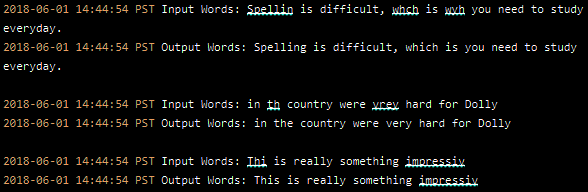
\includegraphics[scale=1]{results_1.png}
\caption{Selected sample from testing}
\label{figR1}
\end{figure}
\FloatBarrier

We are unsure of the lower bound for a two correction passing grade. However, we discovered that the lower bound for three corrections is far above 80 minutes as we could achieve 3 corrections in only a few sentences among tens of thousands of test sentences.

\section{Discussion}
A salient purpose of our model was to demonstrate that one could achieve objectively beneficial results with limited training times. Much of the exact code was an amalgam of templates found on the Tensorflow documentation website and a mixture of different open source codes online. That being said, extensive work was done and can be done to improve the model further. Successful text correction with neural networks has only been around for around 5 years, and it's changing day by day. The prevailing approaches to NLP are already being usurped.

\subsection{Difficulties}
Initially we did not know how long to train the method and it gave really poor results. We began with a training time of about 15 minutes. The results were lackluster at best. A simple sentence like “I drakn wine.” would turn into “Wine wine wine.” Increasing the time to 30 minutes and corrections would begin to occur, but only at the expense of the correct words: “waht is going on?” would become “what is going going?”. After hours of testing, we gathered that the minimally sufficient training time for a passing grade was around 50 minutes. 
\subsection{Improvements}
There are a litany of improvements one could make by optimizing model inputs. However, the single biggest improvement we could make to our model is simply increasing the training time. One particular example is a text corrector developed by Alex Paino which was trained for 2.5 hours and was able to correct they're, their, and there in a sentence \cite{Floyd}. Although Paino's model was optimized for grammar, its results easily surpass the capabilities of our model for text translation. However, a interesting and facile optimization to our model would be to combine it with Paino, perhaps forming an all purpose English corrector.
\subsection{Better Models}
Facebook’s artificial intelligence research (FAIR) team has uncovered a revolutionary way to approach text translation in machine learning models. The basis of this approach is applying a convolution neural network (CNN) instead of a recurrent neural network (RNN) to encode a given data set. The primary benefit of CNN architecture is that it allows a GPU to simultaneously compute all elements of a weight vector rather than sequentially compute them like a RNN does. What this amounts to is a ninefold speed increase compared to the traditional RNN. Thus, despite the fact that we tested our model on a high grade GPU, our RNN approach for text correction cannot fully utilize the capabilities of the hardware. \newline

Despite the speed advantage, researchers have not been able to mimic the performance of a RNN for text translation until FAIR team’s breakthrough. The FAIRs teams text translation approach has a two attributes that allow it to perform well: a multi-hop attention mechanism in the decoding layer and gating \cite{Gehring}. Gating is an already implemented mechanism in RNNs that allows hidden units which store neural network information to pass on specific information to the next hidden unit. For example, gating helps us determine there, their, and they’re in a sentence because the previous words or hidden units in the sentence will clue us in. On the other hand, multi-hop attention mechanism is a boosted version of the attention mechanism we’ve have discussed, which allows the decoder to look at multiple components of the sentence multiple times. In theory this allows the decoder CNN, which already processes information hierarchically, to capture complex relationships by building on top of the base level of sentence components. 

\vspace{1em}

\begin{thebibliography}{7}
\bibitem{Gehring} Gehring, Jonas, et al. “A Novel Approach to Neural Machine Translation.” \emph{Facebook Code}, Facebook, 9 May 2017, \url{code.facebook.com/posts/1978007565818999/a-novel-approach-to-neural-machine-translation/?utm_campaign=Artificial%2BIntelligence%2Band%2BDeep%2BLearning%2BWeekly&utm_medium=email&utm_source=Artificial_Intelligence_and_Deep_Learning_Weekly_13}.

\bibitem{Floyd} Team, FloydHub. “Deep Text Corrector.” \emph{FloydHub Documentation}, \url{docs.floydhub.com/examples/deep_corrector/}.

\end{thebibliography}
\end{document}